\subsection{Métrica geométrica da qualidade da malha}
\label{cap_metrica_geometrica}

\citeonline{Bank97} propõem um algoritmo de suavização e utilizam uma métrica geométrica. Considere $\delta$ o triângulo da figura (\ref{fig_medida_t}), com vértices $v_1$, $v_2$ e $v_3$ e os vetores $ l_1 = \left[ \begin{array}{c}  x_3 - x_2 \\  y_3 - y_2 \end{array} \right ]$, $l_2 = \left[ \begin{array}{c}  x_1 - x_3 \\  y_1 - y_3 \end{array} \right ]$ e $l_3 = \left[ \begin{array}{c}  x_2 - x_1 \\  y_2 - y_1 \end{array} \right ]$, orientados em sentido anti-horário. A medida geométrica, utilizada por \citeonline{Bank97}, chamada {\it Shape Regularity Quality} (SRQ), denotada por $\upsilon(\delta)$, é dada por $\upsilon(\delta) = \frac {4 \sqrt{3}|\delta|} {|l_1|^2 + |l_2|^2 + |l_3|^2}$, em que $2|\delta| = (x_2 - x_3)(y_3 - y_1) - (x_3 - x_1)(y_2 - y_1)$, com os vértices orientados em sentido anti-horário. Caso estejam orientados em sentido horário, o valor de $|\delta|$ será negativo. Trata-se da razão entre a área do triângulo e a soma dos quadrados dos comprimentos das arestas. A constante $4\sqrt{3}$ é utilizada como fator de normalização, para que os valores fiquem entre $0 < \upsilon(\delta) < 1$. Para um triângulo equilátero, $\upsilon(\delta) = 1$, e para triângulos com ângulos muito pequenos será próximo a zero. Para entender o significado geométrico dessa medida, verifique \citeonline{Bank97}. Dada uma malha $M$, a medida SRQ dessa malha é dada pelo menor valor dessa métrica, denominado $\upsilon(\delta)_{min}$.

\begin{figure}[!ht]
  \centering
  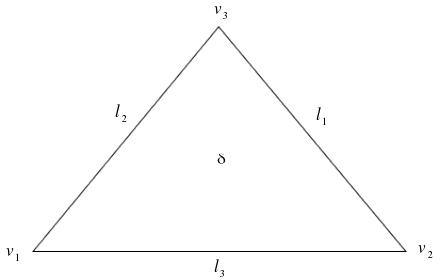
\includegraphics[width=150pt]{imagens_malhas_moveis/medida_t.png}
  \caption{\footnotesize{Rótulos e orientação do triângulo $\delta$.
}}
  \label{fig_medida_t}
\end{figure}

Segundo \citeonline{Bank97}, o único triângulo para o qual $\upsilon (\delta) = 1$ é o triângulo equilátero. Para $\frac{ \sqrt{3} } {2} \leq \upsilon(\delta) \leq 1$ tem-se triângulos sem ocorrência de ângulos obtusos. Conforme $\upsilon(\delta)$ é reduzido, o triângulo $\delta$ se torna mais degenerado.
 
